\documentclass[new,showhints]{nhrproposal}

\newcommand\projecttitle{Benchmark Example}
\newcommand\authors{[PI/PC of the proposal here]}

\begin{document}

  \section{Appendix: Benchmark Example}\label{sec:BenchmarkExample}
\Benchmark{NAMD}
\BenchmarkDescription
  We benchmarked three different systems, characteristic for subproject 1 – 110k atoms, subproject 2 – 240k atoms, and subproject 3 – 500k atoms. Each calculation was performed for 3 hours. The performance is described as ns/day - e.g. the calculated ns divided by 0.125. All calculations are performed with NAMD as described in the code overview section 4.1. In case of the CPU partitions all available cores were used as MPI ranks, while on the GPU system remaining cores were filled with OpenMP threads.

\BenchmarkSystem
Three different resource partitions at the center were used for the benchmarks (md40, std96, grete), in order to determine the most efficient hardware resource to request. In case the most efficient hardware resource is not available, and a different hardware resource than the requested one is granted, this provides information on how to adjust the required resources to perform the planned calculations.
\begin{center}
\begin{tabular}{|G{5cm}|L{3cm}|L{3cm}|L{3cm}|}\hline
  Cluster location & Location 1 & Location 1 & Location 2  \\ \hline
Cluster name & md40 & std96 & grete \\ \hline
  CPUs per node & 2 & 2 & 2 \\ \hline
  CPU type & Intel Xeon Gold  6148 & Intel Xeon Platinum 9242 & AMD EPYC 7315 \\ \hline
Physical CPU-cores per CPU & 20 & 48 & 32 \\ \hline
Main memory per node & 192 GB  & 384 GB & 512 GB \\ \hline
  Interconnect & Omni-Path 100 Gbit/s & Omni-Path  100 Gbit/s & InfiniBand HDR 200 Gbit/s \\ \hline
Accelerators (such as GPUs) &- &- &4x NVIDIA A100 (40 GB)  \\ \hline
\end{tabular}
\end{center}

\BenchmarkData
Performance (ns/day) versus the number of nodes for the three systems we are going to study. The partitions std96, md40 and grete are shown in orange, blue, and red, respectively. The black markers indicate the best performing node combination, while still delivering a parallel efficiency of 70\%:\\
\begin{center}
  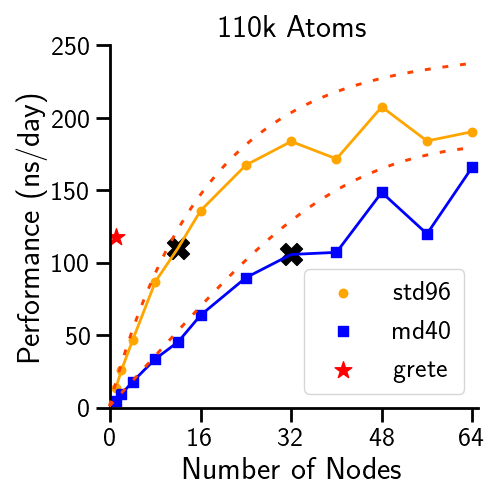
\includegraphics[width=0.27\textwidth]{figures/scaling_110k_atoms_ideal-scaling.png}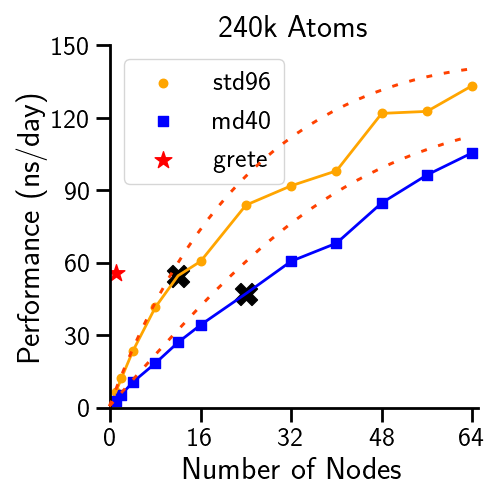
\includegraphics[width=0.27\textwidth]{figures/scaling_240k_atoms_ideal-scaling.png}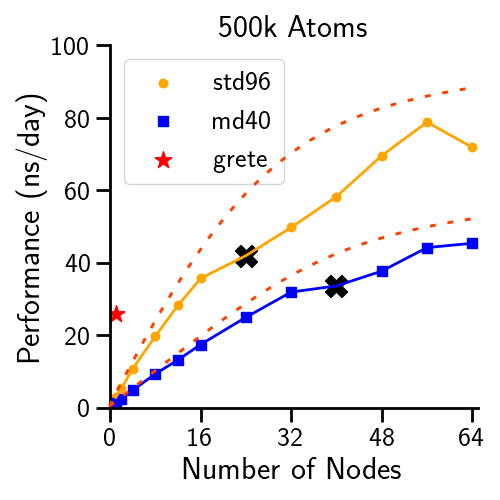
\includegraphics[width=0.27\textwidth]{figures/scaling_500k_atoms_ideal-scaling.png}
\end{center}

\BenchmarkDiscussion
For all the tested systems, the GPU partition grete is most efficient to use, therefore, the performances and costs corresponding to that partition have been printed in bold. For the CPU partitions, we chose the best performing number of nodes, that still delivers a parallel efficiency of 70\%. The resources that we request for the subprojects described in the next section are based on the presented benchmarks. If no GPU resources can be assigned, we would request CPU resources according to the values for the md40 system. md40 performs better than std96 for the 240k and 500k problem sizes, which are overall far more resource intensive than the 100k problem size calculations. The performance difference for the 100k problem size is minor, and for easy of management, it is preferable to have all resources on one system, if the resource impact incurred is minor. 

Comparison of the partitions std96, md40 and grete for three different system sizes in terms of ther performance measures in ns/day and their cost measured in core-h/ns and GPU-h/ns, respectively:
\begin{center}
  \begin{tabular}{l|p{1.5cm}p{1.0cm}p{1.0cm}p{1.5cm}p{2.5cm}|p{2cm}|p{2cm}}
  System &Partition &Cores per Node &GPUs per Node &\# nodes & Performance [ns/day] &Cost [core-h/ns] &Cost [GPU-h/ns] \\ \hline
  100k Atoms &std96 &96  & & 12 &110 &251 & \\
  & md40 & 40 & & 32 & 106 & 290 & \\
    & grete & 64 &4 &1 &\textbf{168} &13 &\textbf{0,8} \\\hline
  240k Atoms &std96 &96 & &12 &55 &502 \\
  &md40 &40 &&24 &47 &490 &\\
    &  grete &64 &4 &1 &\textbf{56} &27 &\textbf{1,7}\\ \hline
  500k Atoms &std96 &96  & &24 &42 &1317 & \\
    &    md40 &40& &40 &34 &1129 & \\
    &grete &64 &4 &1 &\textbf{26} &59 &\textbf{3,7}
\end{tabular}
\end{center}

\end{document}
